\subsubsection{Components Integration and Testing}

In the following section, the order in which the implementation and testing plan are described totally aligns with the order of features presented in the previous chapter.
The aim of this implementation and test plan is to build the \app system in an incremental way, by adding a new feature in every cycle of development, and being able to show the improvements to stakeholders to seek validation.

The main events occurring in the system and the interactions between the various microservices are reported here, classified based on the features presented in the previous section. The purpose of these descriptions is to highlight the particular functionalities that have to be implemented in each component of \app to provide the overall feature and test it, so to detail which parts of the application have to be improved or ignored in each stage of the development.

It is also important to mention the fact that since all communications from the users to the \app platform pass through the Gateway Microservice, this will almost always be involved in the implementation and integration testing of the below features.

\textbf{Login phase, implementation and testing}

The login phase is the entry point of the application. It is primarily handled by the Gateway Microservice, which receives all incoming requests of users and redirects them to the GitHub authentication page. When GitHub verifies the user's credentials, it will send back a message to the Gateway Microservice to inform it of the successful (or unsuccessful) authentication. At that point, the Gateway Microservice sends the username of the user to the User Management Microservice, which verifies whether the user is a new one on the platform of if s/he already has an account. 
The User Management Microservice is also responsible for retrieving all the user's data from the DBMS (if the user already had an account) and building the user interface for showing the personal profile of the user based on that data. If the user is a new one, a new profile is created.

Given these interactions between components of the \app platform, it's pretty straightforward to state that the only microservices that have to be partially implemented to serve the login feature are the Gateway Microservice and the User Management Microservice. 
Here's a schematic representation showing the components involved in this first development cycle and the ones left out.

\begin{center}
	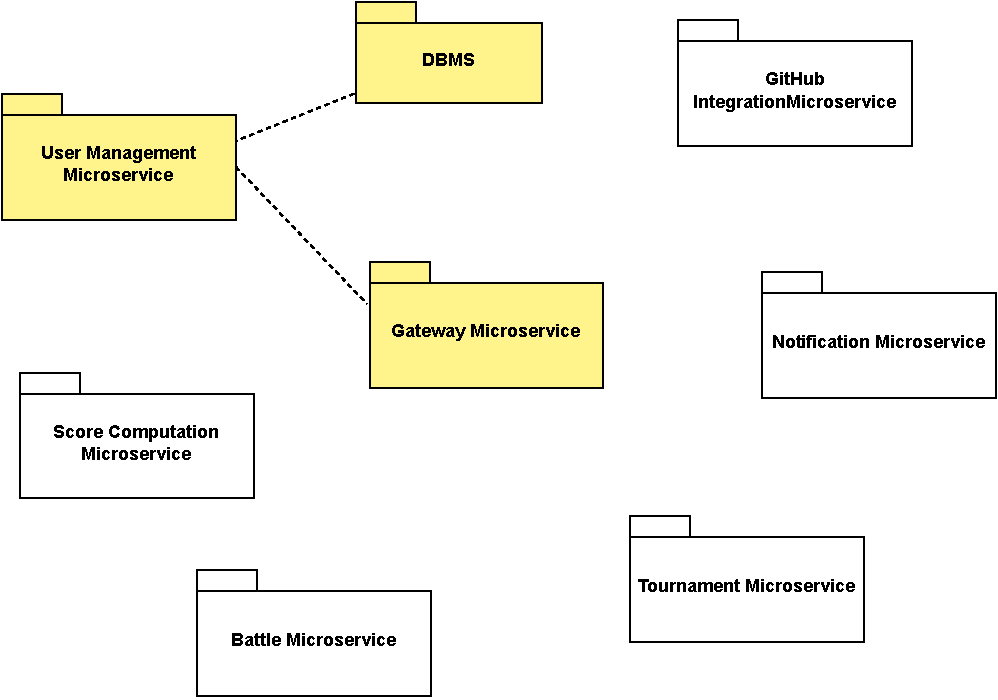
\includegraphics[width=0.6\linewidth, page=1]{1ImplementationPlan_Login}
\end{center}


It has to be noted that inside the Gateway Microservice, only the essential logic to drive the login is going to be implemented, as well as the User Management Microservice will be provided with the logic to handle users' data and build the users' profile interfaces.
Another important point is related to the Discovery Service offered by the Gatway Micrsoervice, which is included as a component to be implemented in this section because all the other features rely on it for the location of microservices.


\textbf{Creation of a new tournament, implementation and testing}

When creating a new tournament, the Gateway Microservice is involved, as it has to intercept the educator's requests and dispatch them to the right microservice, which is in this case the Tournament Microservice. So, part of the Dispatcher component inside the Gateway Microservice has to be implemented. 
The request for the new tournament creation is sent to the Tournament Microservice, which returns the tournament creation form (a user interface), which the Gateway shows to the user.

The educator is now able to fill the form out with the tournament data and confirm. The Gateway Microservice will then forward these pieces of information to the Tournament Microservice which has to create the new tournament in a persistent way (by accessing the DBMS) and then returning the new tournament home page (user interface) to the Gateway Microservice.

Finally, this feature of the application also includes the notifications that have to be sent to all students with an account on CodeKataBattle. As specified in this Design Document, the communications with the Notification Microservice  are handles in an asynchronous way (event-driven programming). Therefore, at this point of the building plan, the event bus has to be built and the Tournament Microservice has to produce a new event every time a tournament is created. 

At the same time, the Notification Microservice is involved, specifically in the process of reading events from the event bus and acting accordingly. At this layer of the implementation, it suffices to implement the logic to respond to the creation of a new tournament, which involves fabricating a new notification for all the students of CodeKataBattle. To do so, the Notification Microservice has to contact the User Management Microservice to retrieve the list of all the users on the platform.

After the tournament has been created on the system, the educator that fabricated the tournament must be able to grant permissions to publish battles to other educators. This feature is internal to the Tournament Microservice.

Finally, students must be able to subscribe to the tournament, which requires the Tournament Microservice to accept requests for tournament participation from the Gateway Microservice.

Here's an illustration of the involved components for this feature.



\begin{center}
	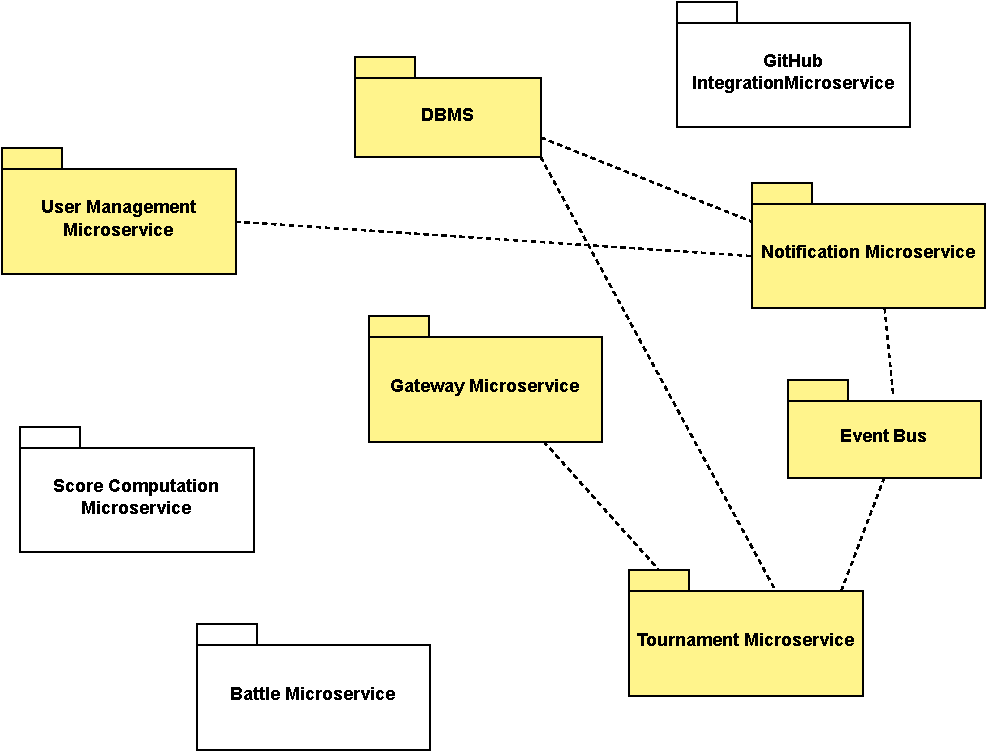
\includegraphics[width=0.6\linewidth, page=1]{2ImplementationPlan_TournamentCreation}
\end{center}


\textbf{3. Creation of a new battle, implementation and testing}

In order to create a new battle, the Battle Microservice has to provide the battle creation form (user interface) through the Gateway. The educator can use the battle creation form to feed the system with all the mandatory data necessary to correctly generate a new battle.

Once the educator confirms his/her choices on the battle creation form, the Gateway Microservice must forward this pieces of information to the Battle Microservice, which will take care of instantiating the new battle in a persistent way (accessing the DBMS).

The next step for the implementation of this feature is the notification of all students subscribed to the tournament in which the battle resides. In order to achieve this:
\begin{itemize}
	\item The Battle Microservice has to publish a new event when the battle is successfully created.
	\item The Notification Microservice listens to the event.
	\item The Notification Microservice leverages the Tournament Microservice to obtain a list of all the students subscribed to the tournament in which the battle resides.
	\item The Notification Microservice produces a notification for all the students in the list
\end{itemize}

Therefore, the Notification Microservice and Tournament Microservice are involved in this step and have to offer these new functionalities.

Moving on, students must be able to join the new battle before the battle registration deadline passes, either as single players or in a team with students. As for the single player mode, this is achieved easily involving only the Battle Microservice, which will receive the student's request through the Gateway.
As for the participation to the battle as a team, students can invite other students to form a team, so the Notification Microservice is involved in this case. The request of a student to invite another student to join a battle together as a team is intercepted by the Gateway Microservice, which dispatches it to the Battle Microservice. The Battle Microservice leverages the Notification Microservice (through the RESTful NotificationAPI) in order to produce an individual notification for the student invited to join the battle in a team.

Finally, the GitHub remote repository dedicated to a battle has to be created when the battle registration deadline passes. In this case, the GitHub Integration Microservice takes care of the task. Once the GitHub repository is created, the GitHub Integration Microservice generates a new event. The Notification Microservices reads the event, contacts the Battle Microservice to obtain a list of all students subscribed to the battle and fabricates the corresponding notifications for all the students on the list.

Here is an illustration of the components involved in the development of this feature, which will be enriched with the functionalities explained above and then tested to see if they integrate and inter-operate to provide the feature of creation of a battle.

\begin{center}
	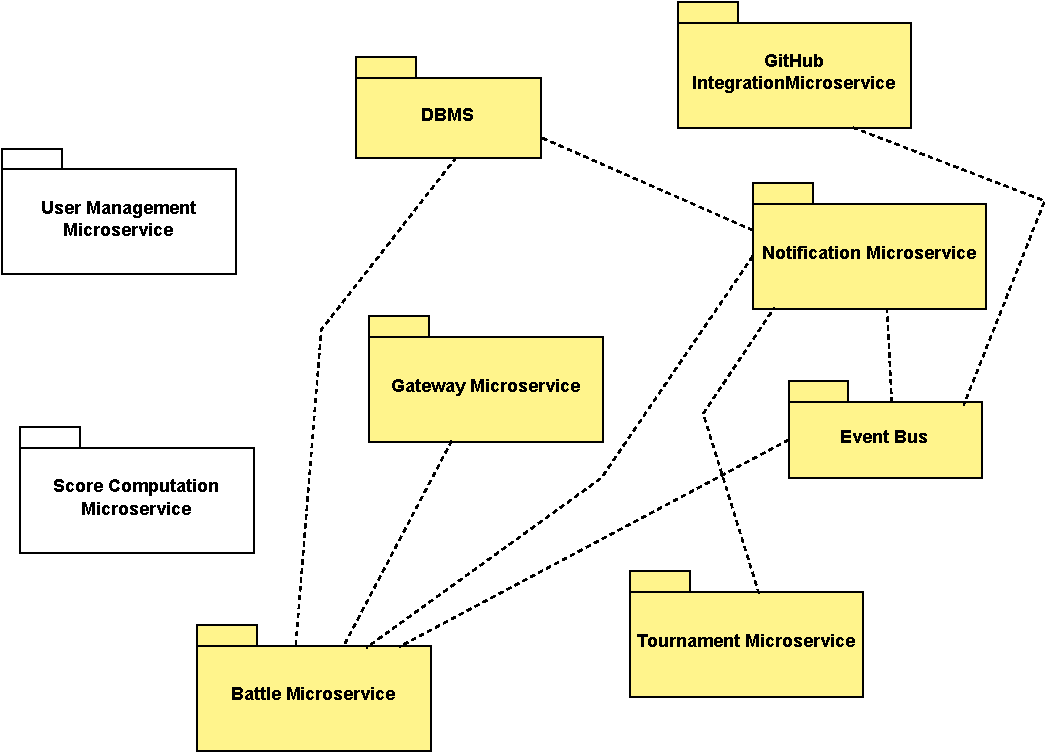
\includegraphics[width=0.6\linewidth, page=1]{3ImplementationPlan_BattleCreation}
\end{center}

\textbf{Pushing Code on GitHub, implementation and testing}

When a student pushes a new code solution on GitHub, many components of the \app platform are involved in a cohesive response to this event.

First, the Gateway Microservice must be always listening to notifications coming from GitHub. Once a new notification arrives, the Gateway Microservice leverages the GitHub Integration Microservice, which takes care of downloading the source code from the correct remote repository and then employs the Score Computation Microservice (through the CalculatorAPI) to compute the score to assign to the solution.

The Score Computation Microservice exploits the interface exposed by the Battle Microservice in order to update the score associated to a team with the new solution provided on GitHub. The ranking of the battle has to be udpated accordingly.

Here's an illustration of the components involved in this specific feature:

\begin{center}
	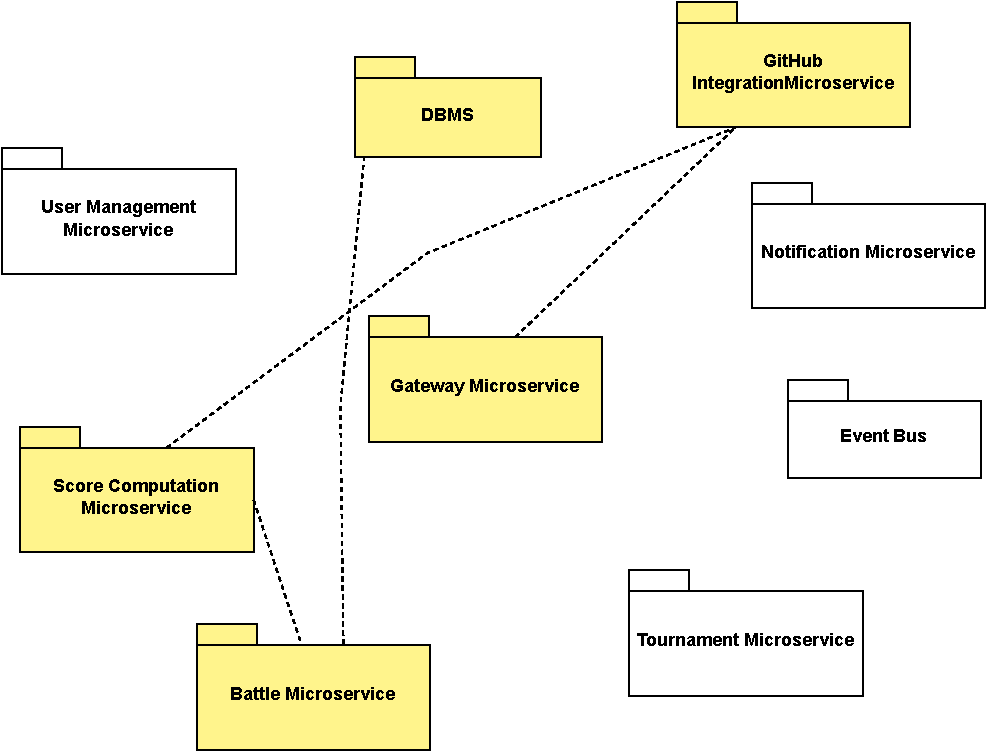
\includegraphics[width=0.6\linewidth, page=1]{4ImplementationPlan_PushSolution}
\end{center}

\textbf{End of a battle, implementation and testing}

The end of a battle first requires the consolidation stage to be handled (if any). The logic for this stage can be integrated in the Battle Microservice.

Then, the battle final ranking has to be published and a notification must be sent to all the students involved in the battle. This implies that the battle has to publish an event and the Notification Microservice has to listen to it. The Notification Microservice then contacts the Battle Microservice to request a list of all students taking part in the battle and fabricates all the notifications accordingly.


Finally, the tournament in which the battle that terminated resides must be updated in terms of its ranking. This is achieved by making the Tournament Microservice listen to the events on the event bus.

Here's an illustration of the components involved and left out in this feature:

\begin{center}
	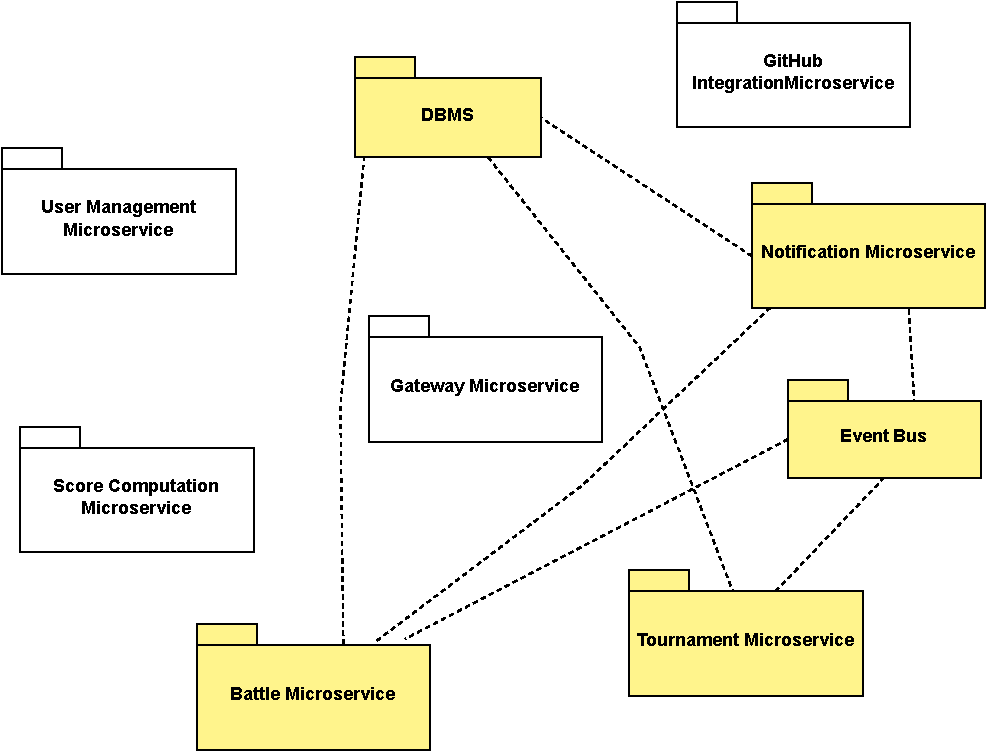
\includegraphics[width=0.6\linewidth, page=1]{5ImplementationPlan_EndBattle}
\end{center}

\textbf{End of a tournament, implementation and testing}

It is only the educator who originally created the tournament to be able to close it. This request is intercepted by the Gateway Microservice, which contacts the Tournament Microservice to close the tournament. 
In turn, the Tournament Microservice will publish an event on the event bus, so that the Notification Microservice can read it, contact again the Tournament Microservice to obtain a list of all students subscribed to the tournament and fabricate a new notification for all of them.

Here's an illustration of the components involved in this feature and of the ones ignored.

\begin{center}
	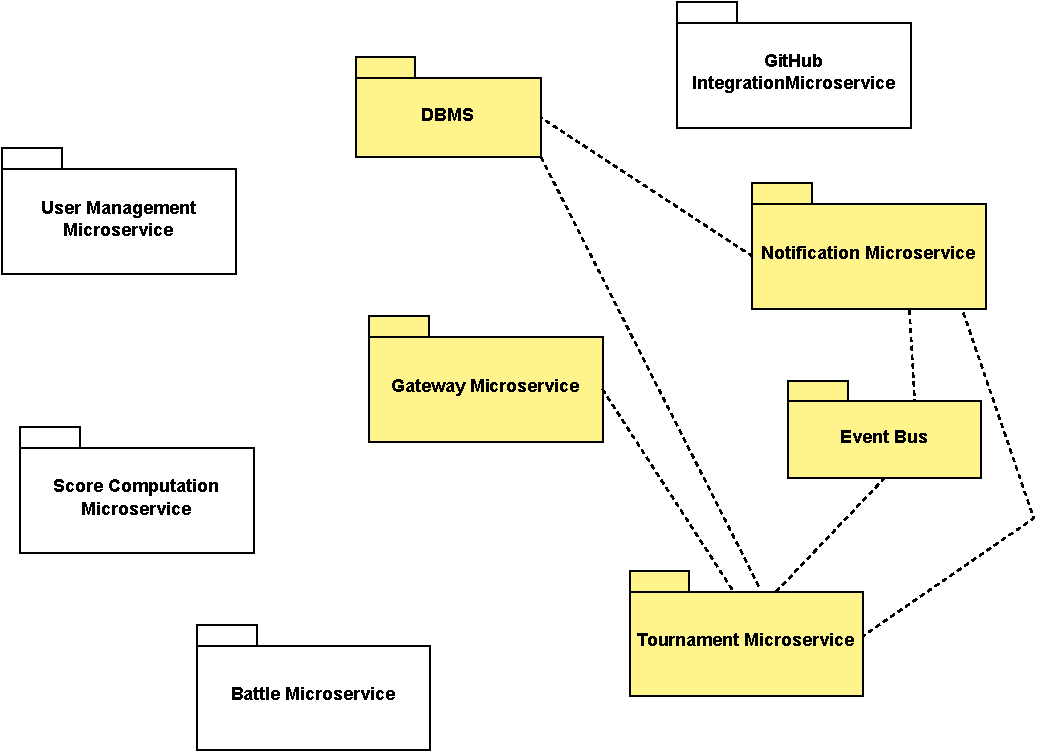
\includegraphics[width=0.6\linewidth, page=1]{6ImplementationPlan_EndTournament}
\end{center}